%------------------------------------------------------------------------------
% Author(s):
% Varaun Ramgoolie
% Copyright:
%  Copyright (C) 2020 Brad Bachu, Arjun Mohammed, Varaun Ramgoolie, Nicholas Sammy
%
%  This file is part of Applied-Mathematics-Unit2 and is distributed under the
%  terms of the MIT License. See the LICENSE file for details.
%
%  Description:
%     Year: 2015
%     Module: 3
%     Question: 6* 
%------------------------------------------------------------------------------

%------------------------------------------------------------------------------
% 6 a
%------------------------------------------------------------------------------

\begin{subquestions}
	
	\subquestion
	We are given a situation where water hits a wall at a certain rate and does not bounce back.
	
	\textbf{\textit{Sketch and Translate:}} \\ \\
	\begin{figure}[H]
		\begin{center}
			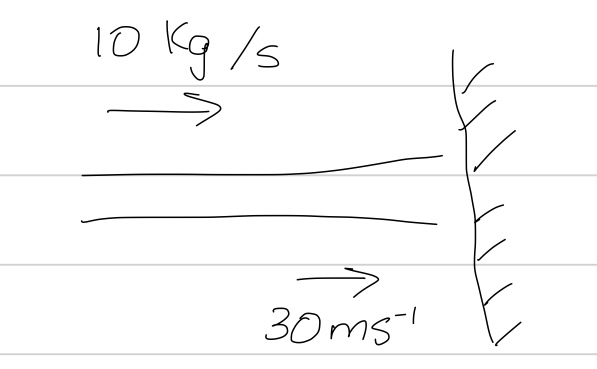
\includegraphics[scale=0.25]{../2015/figures/2015q6-1}
			\caption{\label{2015:q66:fig:Sketch1} Water hitting the wall.}
		\end{center}
	\end{figure}
	We want to find the average force exerted on the wall, given the flow rate of the water and the assumption that the water does not bounce off the wall. We should begin thinking about the relationships that we know with force and the speed/motion of a body.
	
	
	
	
	\textbf{\textit{Simplify and Diagram:}} \\ \\
	\begin{figure}[H]
		\begin{center}
			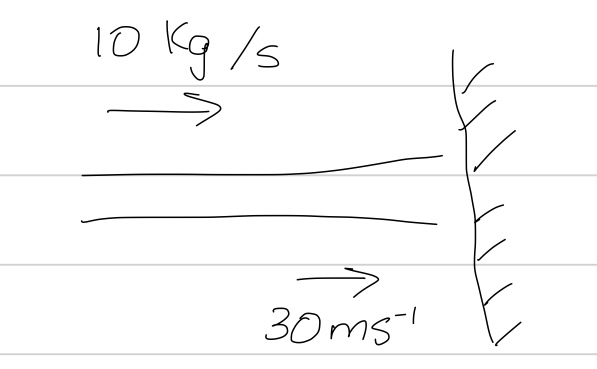
\includegraphics[scale=0.25]{../2015/figures/2015q6-1}
			\caption{\label{2015:q66:fig:Diagram1} Water hitting the wall.}
		\end{center}
	\end{figure}	
	As we are to assume that the water does not bounce off the wall, we can consider the final speed of the water as 0. We are given the flow rate of the water in kgms$^{-1}$ so we should think about equations of force that include a term that looks like $\frac{mass}{time}=\frac{m}{t}$. We shall consider Newton's Second Law. We will also assume that the water is moving in 1 dimension only.
	
	
	
	
	\textbf{\textit{Represent Mathematically:}} \\ \\
	From Newton's Second Law, we know that,
	\begin{equation}
		F=ma \,.
	\end{equation}
	
	If we expand this, we get that,
	\begin{align}
		F & = ma \nn \\
		& = m\frac{(v-u)}{t} \nn \\
		& = \frac{m}{t}(v-u) \,.
	\end{align}
	
	
	
	
	\textbf{\textit{Solve and Evaluate:}} \\ \\
	Considering the moment as the water is about to hit the wall, we get that $u=30$ms$^{-1}$, $v=0$, and $\frac{m}{t}=10$kgs$^{-1}$. Substituting these values, we get that,
	\begin{align}
		F & = \frac{m}{t}(v-u) \nn \\
		& = 10(0-30) \nn \\
		& = -300N \,.
	\end{align}	
	
	As force is a vector, we must be mindful that this value considers the direction from $v$ to $u$. Therefore, the true average force exerted in the direction of $u$ to $v$ is -(-300N) which is 300N.
	
	%------------------------------------------------------------------------------
	% 6 b
	%------------------------------------------------------------------------------
	
	\subquestion
	We are given a situation where a collision occurs and the bodies become coupled after the collision.
	
	\textbf{\textit{Sketch and Translate:}} \\ \\
	\begin{figure}[H]
		\begin{center}
			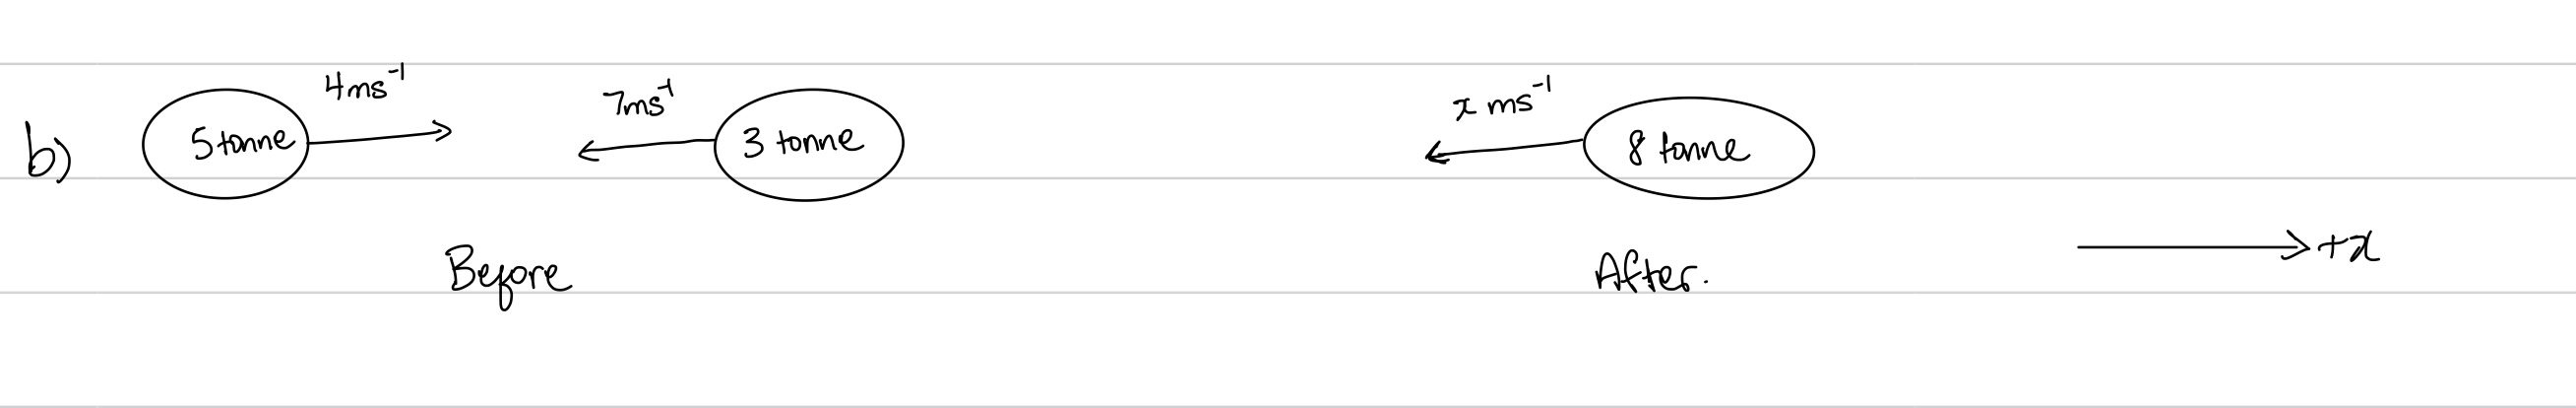
\includegraphics[scale=0.25]{../2015/figures/2015q6-2}
			\caption{\label{2015:q66:fig:Sketch2} Bodies colliding with each other.}
		\end{center}
	\end{figure}	
	We are asked to find the velocity and direction of the coupled body after impact. As we are given the mass and velocities of the bodies, we should begin thinking about what we know about their relationship and the momentum of the bodies.
	
	
	
	
	\textbf{\textit{Simplify and Diagram:}} \\ \\
	\begin{figure}[H]
		\begin{center}
			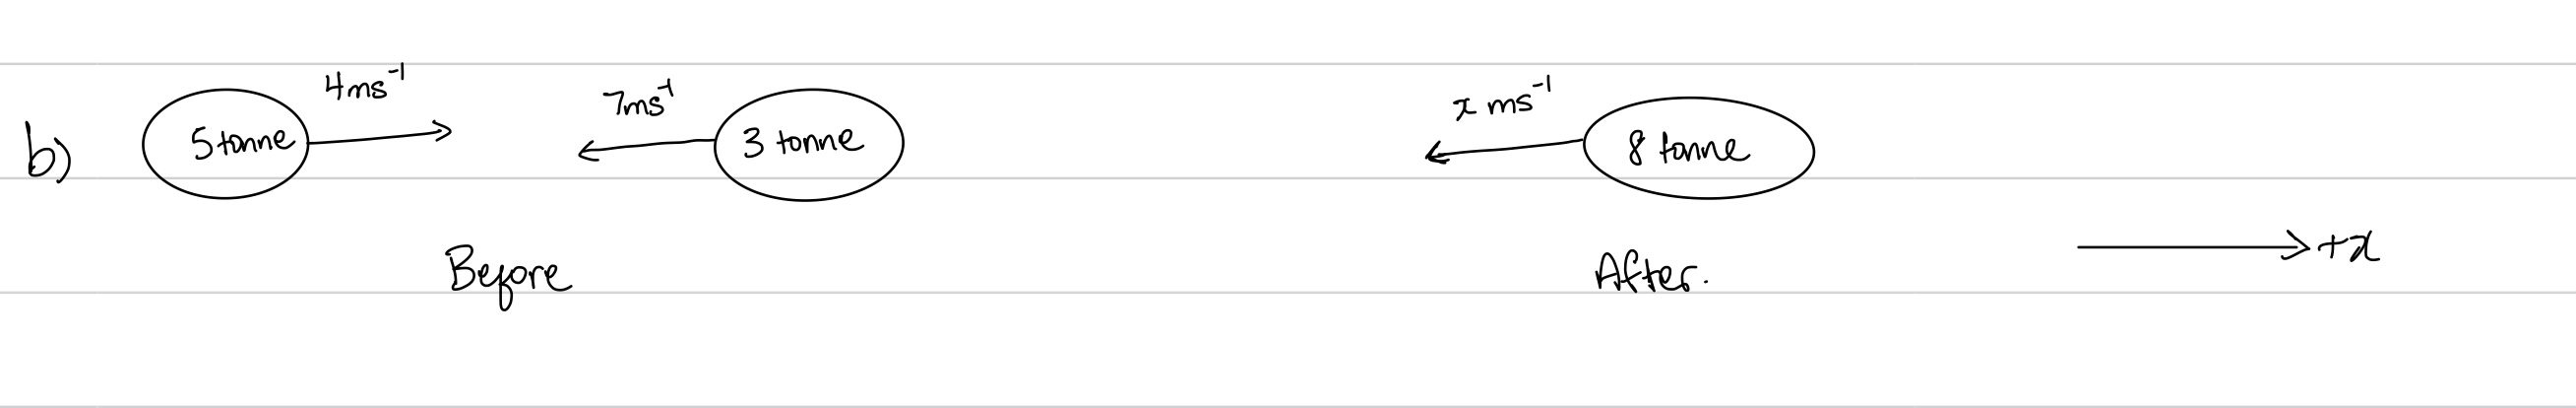
\includegraphics[scale=0.25]{../2015/figures/2015q6-2}
			\caption{\label{2015:q66:fig:Diagram2} Collision overview with velocities and masses.}
		\end{center}
	\end{figure}
	We will assume that the collision occurs in a closed system (no external forces acting on the system). We will take movement to the right as positive and we will assume that the bodies only move in 1 dimension. We can use the Law of Conservation of Momentum to solve this problem.
	
	
	
	
	\textbf{\textit{Represent Mathematically:}} \\ \\
	From the Law of Conservation of Momentum, we get that,
	\begin{align}
		\text{Total Momentum Before collision} & = \text{Total Momentum After collision} \nn \\
		m_1v_1 + m_2v_2 & = (m_1+m_2)v_3 \,.
	\end{align}
	
	
	
	
	\textbf{\textit{Solve and Evaluate:}} \\ \\
	Substituting the values of $m_1=5000$kg, $m_2=3000$kg, $v_1=4$ms$^{-1}$ and $v_2=-7$ms$^{-1}$, we get,
	\begin{align}
		m_1v_1 + m_2v_2 & = (m_1+m_2)v_3 \nn \\
		5000\times4 + 3000\times-7 & = (5000+3000)v_3 \nn \\
		\implies v_3 & = \frac{20000-21000}{8000} \nn \\
		& = \frac{-1}{8}\text{ms}^{-1}
	\end{align}
	The negative sign indicates that the coupled body is moving to the left (as we took the positive direction as to the right).
	
	%------------------------------------------------------------------------------
	% 6 c
	%------------------------------------------------------------------------------
	
	\subquestion
	We are given a pulley system where two masses, are held by a light, inextensible string.
	
	\textbf{\textit{Sketch and Translate:}} \\ \\
	\begin{figure}[H]
		\begin{center}
			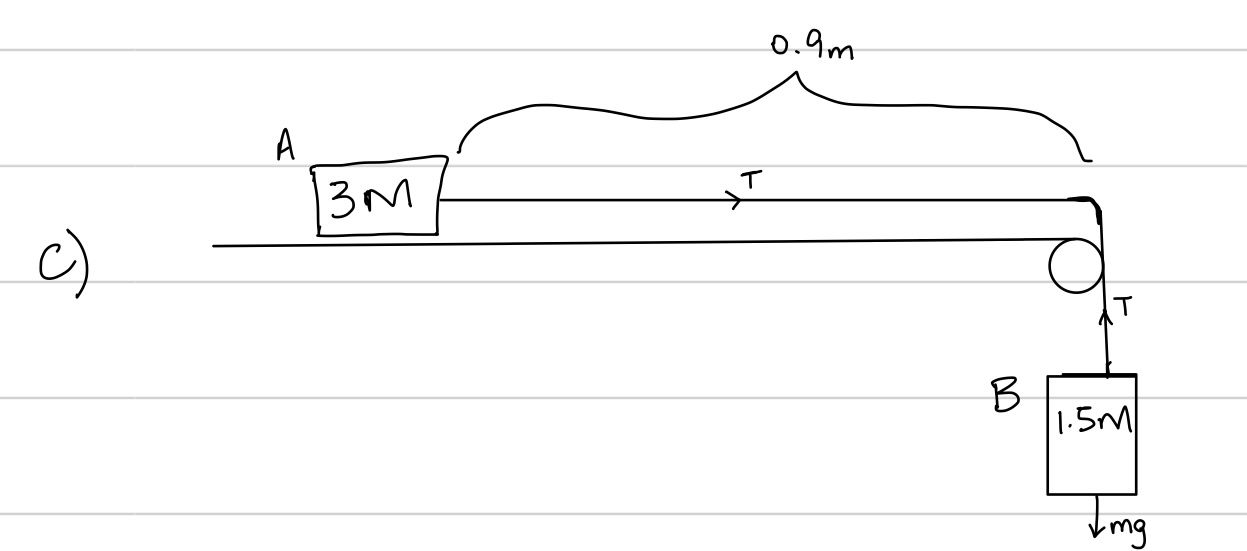
\includegraphics[scale=0.25]{../2015/figures/2015q6-3}
			\caption{\label{2015:q66:fig:Sketch3} Pulley System.}
		\end{center}
	\end{figure}	
	We are asked to find the speed of block A as it reaches the edge of the table. We are given the lengths and dimensions of parts of the system. Contrary to the question's instructions, we will employ a Forces approach to motivate a solution.
	
	
	
	
	\textbf{\textit{Simplify and Diagram:}} \\ \\
	\begin{figure}[H]
		\begin{center}
			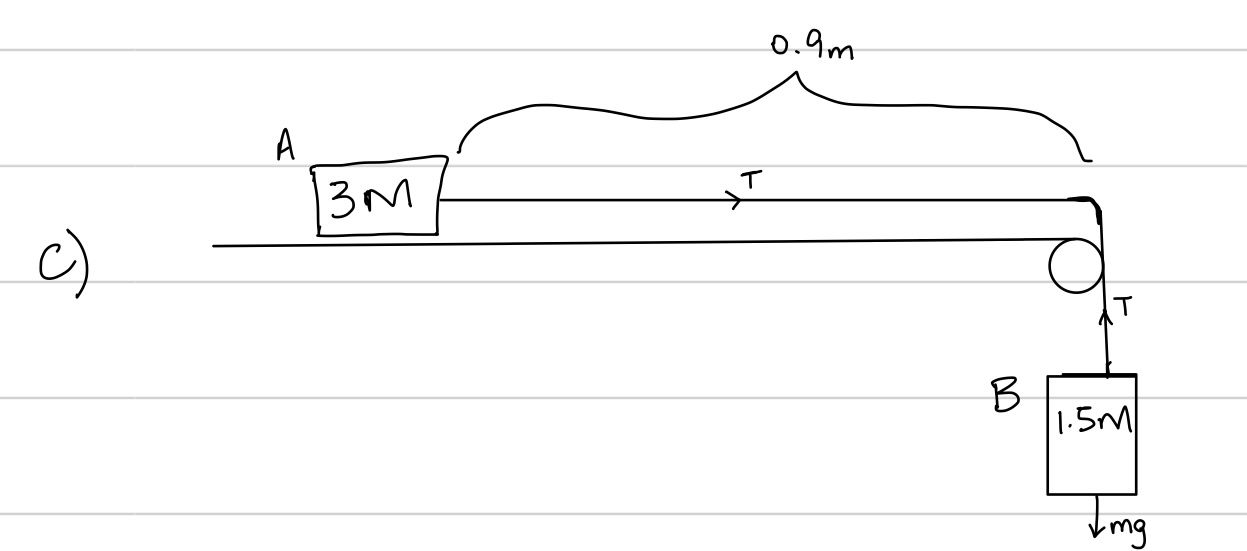
\includegraphics[scale=0.25]{../2015/figures/2015q6-3}
			\caption{\label{2015:q66:fig:Diagram3} Full layout of Pulley System.}
		\end{center}
	\end{figure}
	We will assume that both bodies move in separate 1 dimensional spaces only (A will move in the $+x$ direction and B will move in the $+y$ direction). As the string is light, we can assume that the mass of the string is 0. Similarly, as the string is inextensible, we know that the speed of both particles must be the same (but their velocities will be different due to their movement in perpendicular directions). The acceleration of the bodies must also be the same. We can consider the the tension in the string and solve for the acceleration of both of the particles. We can then use our equations of motion to solve for the velocity of A at the edge of the table.
	
	
	
	
	\textbf{\textit{Represent Mathematically:}} \\ \\
	Considering the 3M mass and using Newton's Second Law in the $+x$ direction, we get that
	\begin{align}
		\sum \vec{F} & = m\vec{a} \nn \\
		T & = 3Ma_x \nn \\ \label{2015:q66:6b1}
	\end{align}
	
	Considering the 1.5M mass and using Newton's Second Law in the $+y$ direction, we get that
	\begin{align}
		\sum \vec{F} & = m\vec{a} \nn \\
		mg-T & = ma_y \nn \\
		1.5Mg - T & = 1.5Ma_y \,. \label{2015:q66:6b2}
	\end{align}
	
	As we mentioned before, the acceleration of the 1.5M and the 3M mass must be the same. Therefore,
	\begin{equation}
		a_x=a_y=a \,.
	\end{equation}

	Finally, we can use our equations of motion to solve for the velocity of $v$ as,
	\begin{align}
		v^2 & = u^2 +2as \nn \\
		\implies v & = \sqrt{u^2+2as} \,.
	\end{align}

	\textbf{\textit{Solve and Evaluate:}} \\ \\
	By solving \req{2015:q66:6b1} and \req{2015:q66:6b2} simultaneously, we get that,
	\begin{align}
		\text{(\req{2015:q66:6b1}+\req{2015:q66:6b1}):} (T)+[1.5Mg-T] & = (3Ma)+[1.5Ma] \nn \\
		1.5Mg & = 4.5Ma \nn \\
		\implies a & = \frac{1}{3}g \text{ms}^{-1} \,.
	\end{align}
	
	Finally, substituting $u=0$(particle released from rest), $s=0.9$m, and $a=\frac{1}{3}g$ms$^{-1}$ into our equation of motion, we get,
	\begin{align}
		v & = \sqrt{u^2+2as} \nn \\
		  & = \sqrt{0+2\times \frac{1}{3}g\times 0.9} \nn \\
		  & = \sqrt{6} \text{ms}^{-1} \,.
	\end{align}
	
	%------------------------------------------------------------------------------
	% 6 c
	%------------------------------------------------------------------------------
	
	\subquestion
	We are given two masses which are connected by a string over a smooth, weightless pulley.
	
	\textbf{\textit{Sketch and Translate:}} \\ \\
	\begin{figure}[H]
		\begin{center}
			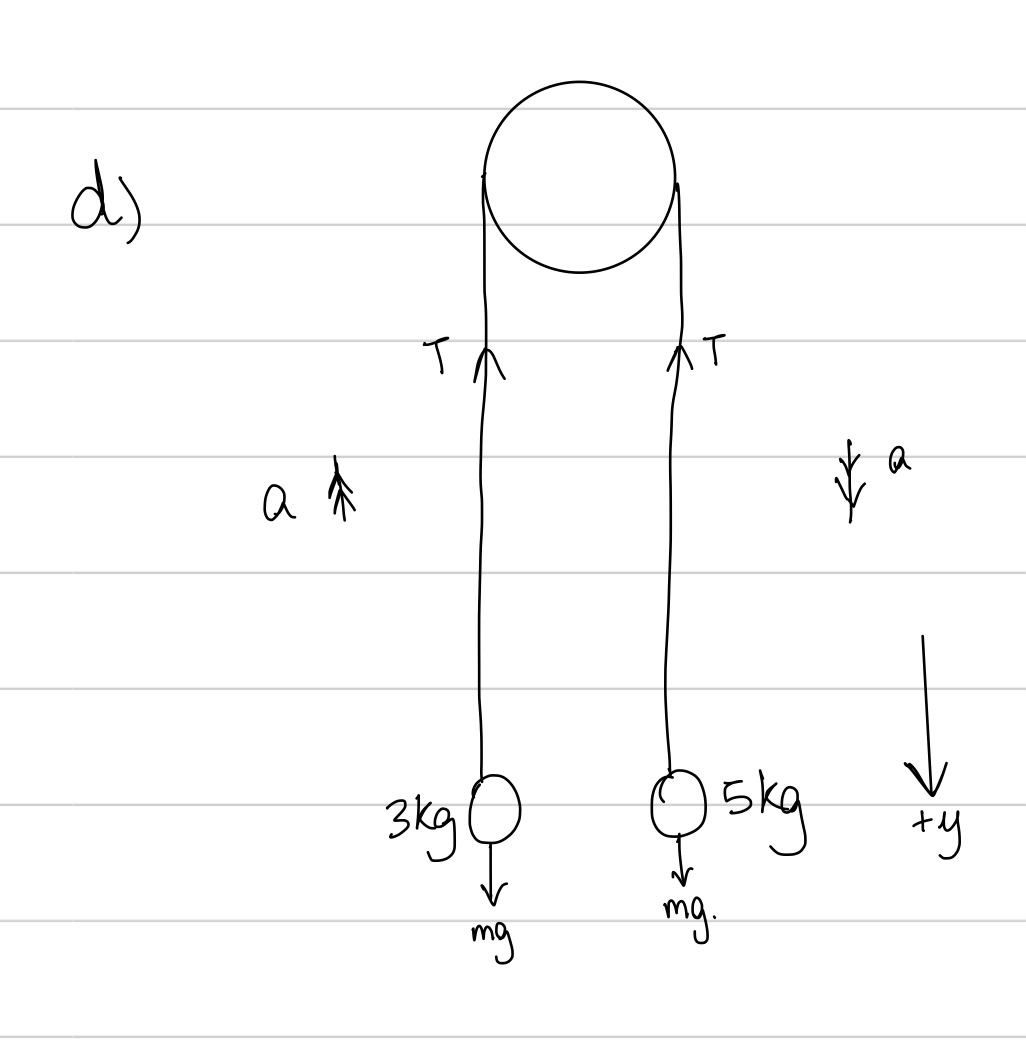
\includegraphics[scale=0.25]{../2015/figures/2015q6-4}
			\caption{\label{2015:q66:fig:Sketch4} Pulley System.}
		\end{center}
	\end{figure}	
	We are asked to find the acceleration of the system given. This problem is a classic pulley problem and so, we should think about what we know about tension and forces in the context of pulleys.
	
	
	
	
	\textbf{\textit{Simplify and Diagram:}} \\ \\
	\begin{figure}[H]
		\begin{center}
			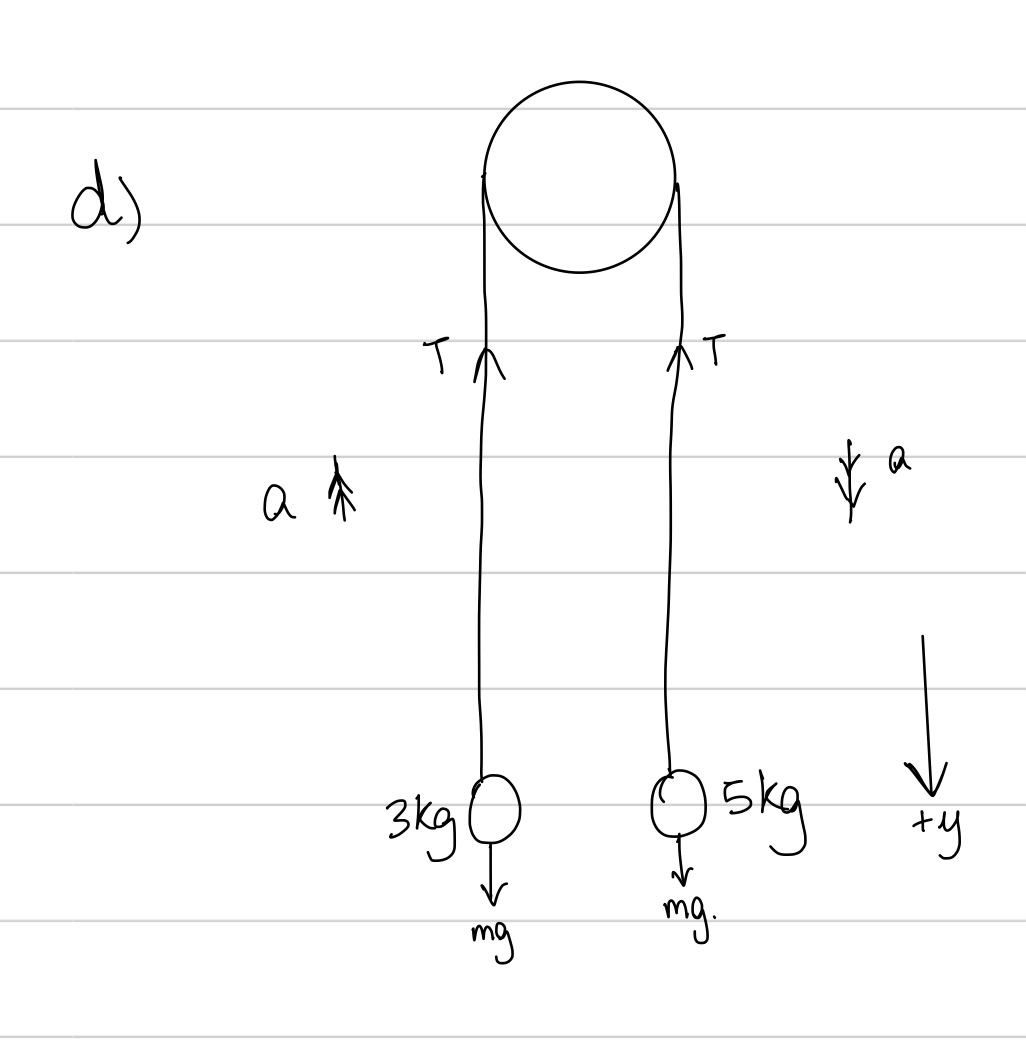
\includegraphics[scale=0.25]{../2015/figures/2015q6-4}
			\caption{\label{2015:q66:fig:Diagram4} All forces on Pulley System.}
		\end{center}
	\end{figure}
	We will assume that both bodies move in only 1 dimension. We will also assume that the mass of the string is 0 and inextensible. Thus, we know that the speed (and acceleration) of both particles must be the same. Since the pulley is smooth, no energy is lost to friction. We should consider how the forces act on the different weights and motivate our solution from there.
	
	
	
	
	\textbf{\textit{Represent Mathematically:}} \\ \\
	Let us first consider the forces on the 5kg mass. From Newton's 2nd Law, we get that,
	\begin{align}
		\sum F & = ma \nn \\
		mg - T & = ma \nn \\
		\implies 5g-T & = 5a \,. \label{2015:q66:PulleyEq1}
	\end{align}
	
	Let us then consider the forces on the 3kg mass. From Newton's 2nd Law, we get that,
	\begin{align}
		\sum F & = ma \nn \\
		T-mg & = ma \nn \\
		\implies T-3g & = 3a \,. \label{2015:q66:PulleyEq2}
	\end{align}
	
	
	
	
	\textbf{\textit{Solve and Evaluate:}} \\ \\
	By solving \req{2015:q66:PulleyEq1} and \req{2015:q66:PulleyEq2} simultaneously, we get,
	\begin{align}
		\text{(\req{2015:q66:PulleyEq1}+\req{2015:q66:PulleyEq2}):} (5g-T)+[T-3g] & = (5a)+[3a] \nn \\
		2g & = 8a \nn \\
		\implies a & = \frac{1}{4}g = 2.5\text{ms}^{-2} \,.
	\end{align}
	
	
	
	
\end{subquestions}